\section{Teoria}
\subsection{Wybór mezonu}

\begin{figure}[H]
\centering
\includegraphics[width=.5\textwidth]{./img/Rysunek}
\caption{Diagram Feynmana rozpadu mezonu K$^0_\text{S}$}
\label{img:feynman}
\end{figure}

Wybrany przez autorów mezon to kaon K$^0_\text{S}$. Proces rozpadu kaonu zachodzi przez oddziaływanie słabe, w tym przypadku
kwark $\bar{\text s}$ rozpada się na $\bar{\text u}$ z emisją bozonu W$^+$.
Diagram Feynmana rozpadu tej cząstki na piony $\pi^+$ i $\pi^-$ przedstawiony został na rysunku~\ref{img:feynman}.
Zauważyć można, że z kwarków wyjściowych powstać mogły też piony $\pi^0$ (d$\bar{\text d}$ i u$\bar{\text u}$), jednak 
prawdopodobieństwo na ten rozpad (30\%\cite{database:K}) jest dużo mniejsze od prawdopodobieństwa na rozpad 
$\pi^+$ i $\pi^-$ (69\%\cite{database:K}) ze względu na tłumienie przez kolor.

\subsection{Sposób obliczeń}
W celu wykonania histogramu masy mezonu wykorzystano bezpośrednio zmienną D\_Ks0\_M zawartą w drzewie. Do wyliczenia czasu życia posłużono się wzorem

\begin{equation}
\tau = \frac{m d}{p c}\ ,
\end{equation}

gdzie $m$ - masa, $d$ - przebyty dystans a $p$ - wartość pędu cząstki. Pęd uzyskano bezpośrednio ze zmiennej D\_Ks0\_P w drzewie, zaś $d$ wyliczono na podstawie współrzędnych wierzchołka początkowego i końcowego.

\subsection{Kryteria wyboru przypadków sygnałowych}
%\textcolor{red}{Ja tu nie wiem co napisać :D}
W celu wybrania przypadków zapewniających lepszą dokładność wyników zastosowano selekcję poprzez wybór zdarzeń, dla których dodatkowe zmienne mieszczą się w odpowiednich zakresach:
\begin{itemize}
\item parametr zderzenia w wierzchołku produkcji - powinien być jak najmniejszy dla cząstki wytworzonej w tym wierzchołku,
\item wartość $\chi^2$ parametru zderzenia w wierzchołku produkcji - jak najmniejsza,
\item flight distance - wybierane parametry z jak największym.
\end{itemize}

Dodatkowo, do wyznaczenia czasu życia wykorzystano przypadki pozostałe po odrzuceniu gaussowskiego ogona rozkładu masy.